\documentclass[11pt, a4paper]{article}

\usepackage[margin=1in]{geometry}
\usepackage{booktabs}
\usepackage{graphicx}
\usepackage{amsmath}
\usepackage{amssymb}
\usepackage{hyperref}
\usepackage{xcolor}
\usepackage{caption}
\usepackage{subcaption}
\usepackage{array}
\usepackage{parskip}
\usepackage{enumitem}
\usepackage{titlesec}

\hypersetup{
    colorlinks=true,
    linkcolor=blue!60!black,
    citecolor=blue!60!black,
    urlcolor=blue!60!black,
}

\titleformat{\section}{\large\bfseries}{}{0em}{\thesection.\quad}
\titleformat{\subsection}{\normalsize\bfseries}{}{0em}{\thesubsection\quad}

\title{\textbf{Behavioral Clustering of Kalshi Sports Prediction Markets}\\[0.4em]
\large Methodology and Findings Report}
\author{William Walz \and Indigo Lee\\[0.3em]
\small Claremont Graduate University --- Math 364: Machine Learning in Asset Pricing}
\date{}

\begin{document}

\maketitle

\begin{abstract}
We apply unsupervised machine learning to 946 resolved Kalshi sports prediction markets to ask whether price dynamics — independent of sport or market type — cluster into distinct behavioral patterns. From hourly candlestick data, we engineer eight features per market capturing final price level, short-term momentum, lifetime range, volatility, drift, duration, and time spent near the 50\% threshold. K-means clustering ($k=4$, selected by silhouette score) identifies four behaviorally distinct groups: stable underdogs, late-converging favorites, volatile near-misses, and long-duration series markets. We find that these clusters cut across Kalshi's own market taxonomy — game winners and player props occupy the same behavioral clusters. A two-sided binomial calibration test finds no statistically significant mispricing in any cluster (all $p > 0.22$), suggesting Kalshi's crowd forecasts are well-calibrated despite behavioral variation in price paths.
\end{abstract}

\tableofcontents
\vspace{1em}

% ─────────────────────────────────────────────────────────────────────────────
\section{Introduction and Research Questions}

Kalshi is a regulated prediction market exchange where traders buy and sell binary contracts that pay \$1 if an event occurs and \$0 otherwise. Contract prices therefore represent crowd-aggregated probability estimates. Sports markets on Kalshi span game outcomes, player performance thresholds, team totals, and multi-game series results — each with distinct information environments and resolution timelines.

This project investigates two questions:

\begin{enumerate}[noitemsep]
  \item \textbf{Behavioral clustering:} Do Kalshi sports markets organize into natural behavioral types based solely on their pre-resolution price dynamics, and do those types align with Kalshi's stated market-type taxonomy or cut across it?
  \item \textbf{Calibration:} Are some behavioral types systematically mispriced — i.e., does the crowd's final price consistently overestimate or underestimate the actual resolution probability for markets in certain behavioral clusters?
\end{enumerate}

The study is purely observational. We use no fundamental information about teams, players, or game outcomes beyond what is embedded in the price history itself.

% ─────────────────────────────────────────────────────────────────────────────
\section{Data Collection}

\subsection{API Source}
All data was collected from the Kalshi REST API v2 (\texttt{https://api.elections.kalshi.com/trade-api/v2}). The API is publicly accessible without authentication for settled markets. Market listings were retrieved using the \texttt{/markets} endpoint with \texttt{status=settled} and cursor-based pagination to collect all resolved contracts.

\subsection{Market Selection}
We targeted NBA basketball markets from 24 series covering the 2024--25 season, including game winners, player points/assists/rebounds props, team totals, halftime totals, point spreads, and series outcomes. A total of \textbf{19,406 unique resolved markets} were collected across all series, stored in \texttt{data/raw\_markets.csv}.

\subsection{Price History Collection}
Hourly candlestick data (OHLCV) was collected for each market via:
\begin{center}
\texttt{/series/\{series\_ticker\}/markets/\{market\_ticker\}/candlesticks?period\_interval=60}
\end{center}
Each candlestick represents a 1-hour window. Prices are denominated in cents (0--100), representing probability in \%. To limit API load, we used stratified sampling: up to 300 markets per \texttt{market\_type}, collecting candlesticks only for markets with \texttt{duration\_hours} $\geq 24$. This yielded \textbf{49,015 candlestick records} across 996 markets, stored in \texttt{data/raw\_price\_history.csv}.

\subsection{Raw Data Schema}

\begin{table}[h!]
\centering
\caption{Key fields in \texttt{data/raw\_markets.csv} (19,406 rows)}
\begin{tabular}{lll}
\toprule
Field & Type & Description \\
\midrule
\texttt{market\_id} & string & Unique market identifier \\
\texttt{series\_ticker} & string & Parent series (e.g., \texttt{NBA-2025-BOS}) \\
\texttt{market\_type} & string & Category (game\_winner, player\_points, etc.) \\
\texttt{result} & string & Resolution: \texttt{"yes"} or \texttt{"no"} \\
\texttt{open\_time} & datetime & Market open timestamp \\
\texttt{close\_time} & datetime & Market close timestamp \\
\texttt{duration\_h} & float & Lifetime in hours \\
\bottomrule
\end{tabular}
\end{table}

% ─────────────────────────────────────────────────────────────────────────────
\section{Feature Engineering}

\subsection{Notation}
Let $\mathbf{p} = (p_1, p_2, \ldots, p_T)$ denote the sequence of hourly closing prices (in probability space, $p_t \in [0,1]$) for a given market, where $T$ is the total number of observed candles.

\subsection{Eight Behavioral Features}

We compute the following features from each market's price history:

\vspace{0.5em}

\noindent\textbf{1. Final probability} (\texttt{final\_prob}): The closing price at the last observed candle — the market's best consensus estimate just before resolution.
\[
\texttt{final\_prob} = p_T
\]

\noindent\textbf{2. Three-hour price change} (\texttt{change\_3h}): Price momentum in the final 3 hours.
\[
\texttt{change\_3h} = \begin{cases} p_T - p_{T-3} & \text{if } T \geq 4 \\ p_T - p_1 & \text{otherwise} \end{cases}
\]

\noindent\textbf{3. Twenty-four-hour price change} (\texttt{change\_24h}): Price momentum in the final 24 hours — the single most informative window for late-breaking information.
\[
\texttt{change\_24h} = \begin{cases} p_T - p_{T-24} & \text{if } T \geq 25 \\ p_T - p_1 & \text{otherwise} \end{cases}
\]

\noindent\textbf{4. Total range} (\texttt{total\_range}): The maximum price excursion over the market's lifetime — captures how contested the outcome was at any point.
\[
\texttt{total\_range} = \max(\mathbf{p}) - \min(\mathbf{p})
\]

\noindent\textbf{5. Volatility} (\texttt{volatility}): Standard deviation of hourly price increments — captures intraday noisiness independent of directional drift.
\[
\texttt{volatility} = \mathrm{std}\!\left(\Delta p\right), \quad \Delta p_t = p_t - p_{t-1}
\]

\noindent\textbf{6. Drift slope} (\texttt{drift\_slope}): The OLS slope $\hat{\beta}$ from regressing closing prices on time over the final 24 candles (or full history if $T < 24$). A positive slope means the market was trending toward YES; negative toward NO.
\[
p_t = \alpha + \beta t + \varepsilon_t, \quad \hat{\beta} = \texttt{drift\_slope}
\]

\noindent\textbf{7. Days open} (\texttt{days\_open}): Total market lifetime in days.
\[
\texttt{days\_open} = \frac{\text{duration\_hours}}{24}
\]

\noindent\textbf{8. Time near 50\%} (\texttt{time\_near\_50}): Fraction of lifetime that the market spent within $[0.40, 0.60]$ — the ``contested zone.'' Markets with high values were genuinely uncertain for extended periods.
\[
\texttt{time\_near\_50} = \frac{\left|\{t : 0.40 \leq p_t \leq 0.60\}\right|}{T}
\]

\subsection{Data Funnel}

\begin{table}[h!]
\centering
\caption{Row counts at each pipeline stage}
\begin{tabular}{lrl}
\toprule
Stage & Markets & Filter applied \\
\midrule
Raw markets & 19,406 & All settled NBA markets \\
With price history & 996 & $\geq 2$ candlestick records \\
After preprocessing & 946 & duration $\geq 24$h, $n_\text{obs} \geq 10$, no NaN features \\
Cluster summaries & 4 & One row per cluster \\
\bottomrule
\end{tabular}
\end{table}

% ─────────────────────────────────────────────────────────────────────────────
\section{Preprocessing and Normalization}

\subsection{Filtering}
Before clustering, markets were filtered to remove:
\begin{itemize}[noitemsep]
  \item Markets with \texttt{duration\_hours} $< 24$ — too short to capture meaningful price dynamics.
  \item Markets with fewer than 10 price observations (\texttt{n\_obs} $< 10$) — insufficient history for reliable feature computation.
  \item Markets with \texttt{NaN} in any of the 8 feature columns — typically caused by degenerate price histories (e.g., constant price throughout).
\end{itemize}
These filters reduced the dataset from 996 to \textbf{946 markets}.

\subsection{Z-Score Normalization}
K-means clustering partitions points by minimizing within-cluster sum of squared Euclidean distances. This means features with large numeric ranges dominate the distance calculation. In our dataset, \texttt{days\_open} ranges from approximately 1 to 30+, while \texttt{volatility} ranges from 0 to 0.05. Without normalization, a 5-day difference in \texttt{days\_open} would swamp a 0.05 difference in \texttt{volatility}, even if volatility carries more discriminative signal.

We apply \textbf{StandardScaler} (sklearn) to all 8 features independently:
\[
z_{i,j} = \frac{x_{i,j} - \mu_j}{\sigma_j}
\]
where $x_{i,j}$ is feature $j$ for market $i$, $\mu_j$ is the feature mean, and $\sigma_j$ is the feature standard deviation across all 946 markets. After scaling, each feature has mean 0 and standard deviation 1 across the dataset.

% ─────────────────────────────────────────────────────────────────────────────
\section{Clustering Methodology}

\subsection{Algorithm: K-Means}
We use Lloyd's k-means algorithm as implemented in \texttt{sklearn.cluster.KMeans} with \texttt{n\_init=10} (ten independent random restarts, keeping the best inertia) and \texttt{random\_state=42} for reproducibility.

K-means minimizes the within-cluster sum of squared distances (inertia):
\[
\text{Inertia} = \sum_{k=1}^{K} \sum_{i \in C_k} \|\mathbf{z}_i - \boldsymbol{\mu}_k\|^2
\]
where $C_k$ is the set of points assigned to cluster $k$ and $\boldsymbol{\mu}_k$ is the cluster centroid.

\subsection{Selecting $k$: Elbow Curve and Silhouette Score}
We fit models for $k \in \{2, 3, 4, 5, 6, 7\}$ and evaluate each using two criteria:

\begin{enumerate}[noitemsep]
  \item \textbf{Elbow curve}: Plot inertia vs.\ $k$. The ``elbow'' — where marginal inertia reduction flattens — suggests a natural stopping point.
  \item \textbf{Silhouette score}: For each point $i$, let $a(i)$ be the mean distance to other points in its cluster and $b(i)$ be the mean distance to points in the nearest other cluster:
  \[
  s(i) = \frac{b(i) - a(i)}{\max(a(i),\, b(i))}, \quad s(i) \in [-1, 1]
  \]
  The dataset silhouette score is $\bar{s} = \frac{1}{n}\sum_i s(i)$. Higher is better.
\end{enumerate}

\begin{figure}[h!]
\centering
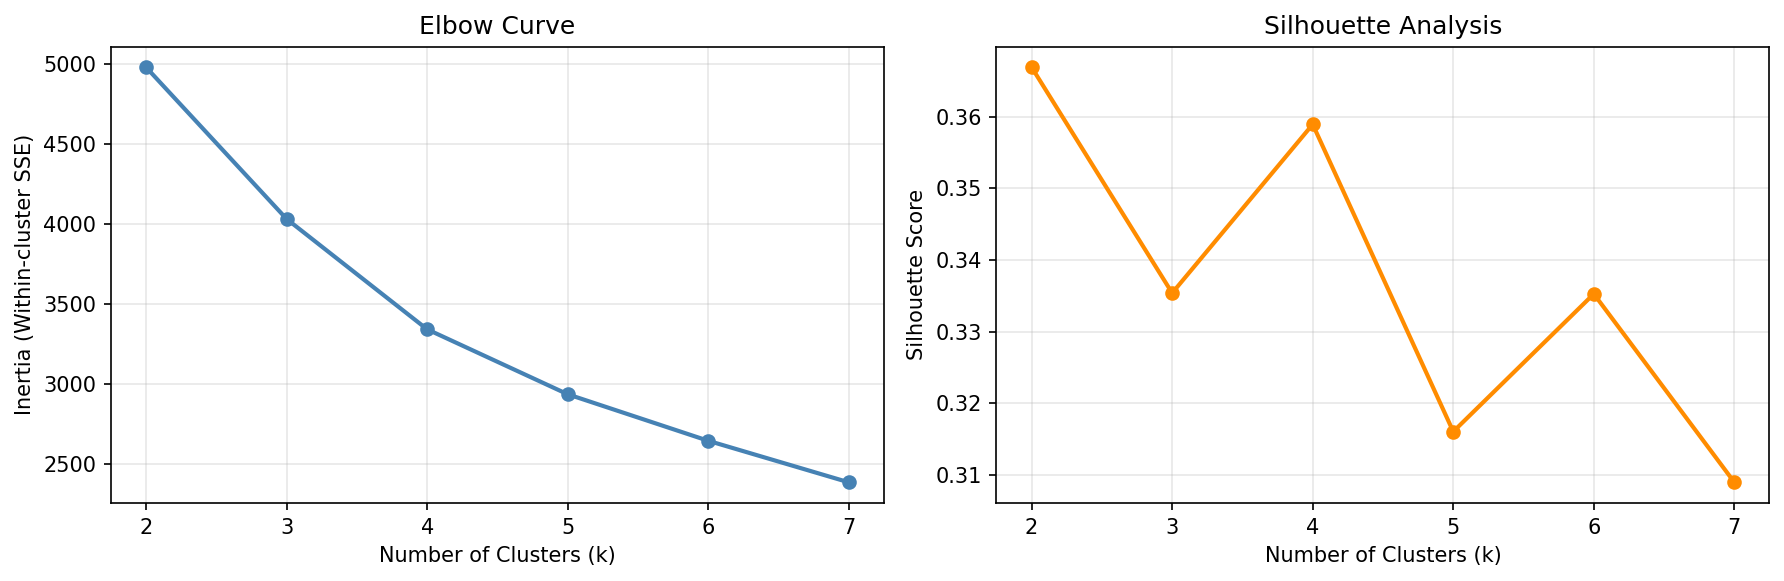
\includegraphics[width=0.85\textwidth]{elbow_curve.png}
\caption{Elbow curve (left) and silhouette scores (right) for $k = 2$ through $7$.}
\end{figure}

The global silhouette maximum occurs at $k=2$ (separating YES-side from NO-side markets). While statistically optimal, $k=2$ is behaviorally trivial — it simply recapitulates the binary outcome structure. We enforce a minimum of $k=4$ to require the model to find richer within-outcome variation, and select the $k \geq 4$ value with the highest silhouette score.

\textbf{Result: $k=4$ selected} (silhouette $= 0.3589$), representing a meaningful behavioral decomposition with reasonable cluster cohesion.

% ─────────────────────────────────────────────────────────────────────────────
\section{Results: Cluster Characterization}

\subsection{Overview}

\begin{table}[h!]
\centering
\caption{Cluster summary statistics}
\begin{tabular}{crrrrrl}
\toprule
Cluster & $n$ & Avg.\ Final Prob & YES Rate & Mispricing & Dom.\ Type & Label \\
\midrule
0 & 453 & 16.3\% & 14.1\% & $-$2.1 pp & half\_spread & Stable underdog \\
1 & 286 & 85.4\% & 83.9\% & $-$1.5 pp & team\_total & Late-converging favorite \\
2 & 177 & 13.8\% & 15.8\% & $+$2.0 pp & half\_total & Volatile near-miss \\
3 &  30 & 32.8\% & 26.7\% & $-$6.1 pp & series\_outcome & Long-duration series \\
\bottomrule
\end{tabular}
\end{table}

\subsection{Cluster Descriptions}

\textbf{Cluster 0 --- Stable Underdog ($n=453$):}
These markets were consistently priced below 25\% throughout their lifetimes, with almost no time spent near the 50\% threshold (mean \texttt{time\_near\_50} = 2\%). Volatility is low (mean $\sigma_{\Delta p} = 0.040$), indicating the crowd saw the outcome as largely predetermined from market open. They resolved NO 86\% of the time. This is the largest cluster and is dominated by spread and total markets where one side was heavily favored.

\textbf{Cluster 1 --- Late-Converging Favorite ($n=286$):}
These markets had a large 24-hour price change (mean $+0.48$) and the widest total range (mean 0.73), indicating that markets started ambiguous and converged decisively to a high probability in the final day. They resolved YES 84\% of the time. The dominant market type is \texttt{team\_total}. These are markets where the outcome became clear only close to resolution — perhaps after a game or quarter was in progress.

\textbf{Cluster 2 --- Volatile Near-Miss ($n=177$):}
These markets spent 46\% of their lifetime near 50\% before ultimately resolving NO 84\% of the time. They exhibit a strong negative 24-hour drift (mean $-0.29$) and a wide total range (mean 0.59). The crowd appeared genuinely uncertain throughout most of the market's life, then shifted decisively toward NO shortly before resolution. These are the most interesting markets from a price discovery standpoint.

\textbf{Cluster 3 --- Long-Duration Series ($n=30$):}
These markets were open for an average of 14 days — far longer than any other cluster. They are dominated by \texttt{series\_outcome} contracts (e.g., who wins a best-of-7 series). Low short-term volatility (mean $\sigma_{\Delta p} = 0.046$) reflects gradual updating over many games rather than single-event jumps. The YES rate (26.7\%) is below the final price (32.8\%), though this is not statistically significant given the small sample.

\subsection{Visualizations}

\begin{figure}[h!]
\centering
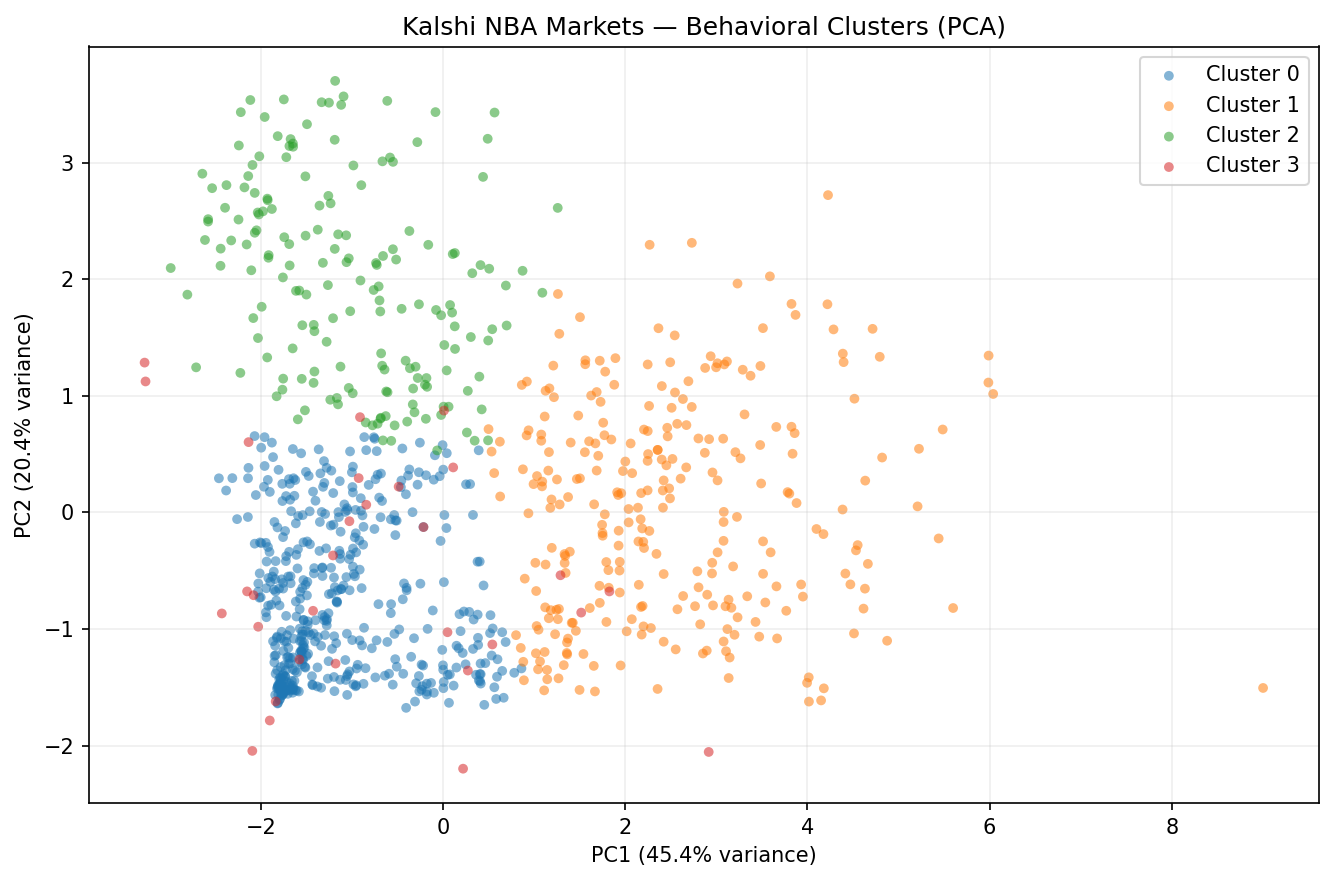
\includegraphics[width=\textwidth]{cluster_scatter.png}
\caption{PCA projection of all 946 markets onto the first two principal components, colored by cluster assignment. The two PCs capture the dominant axes of variation in the 8-dimensional feature space.}
\end{figure}

\begin{figure}[h!]
\centering
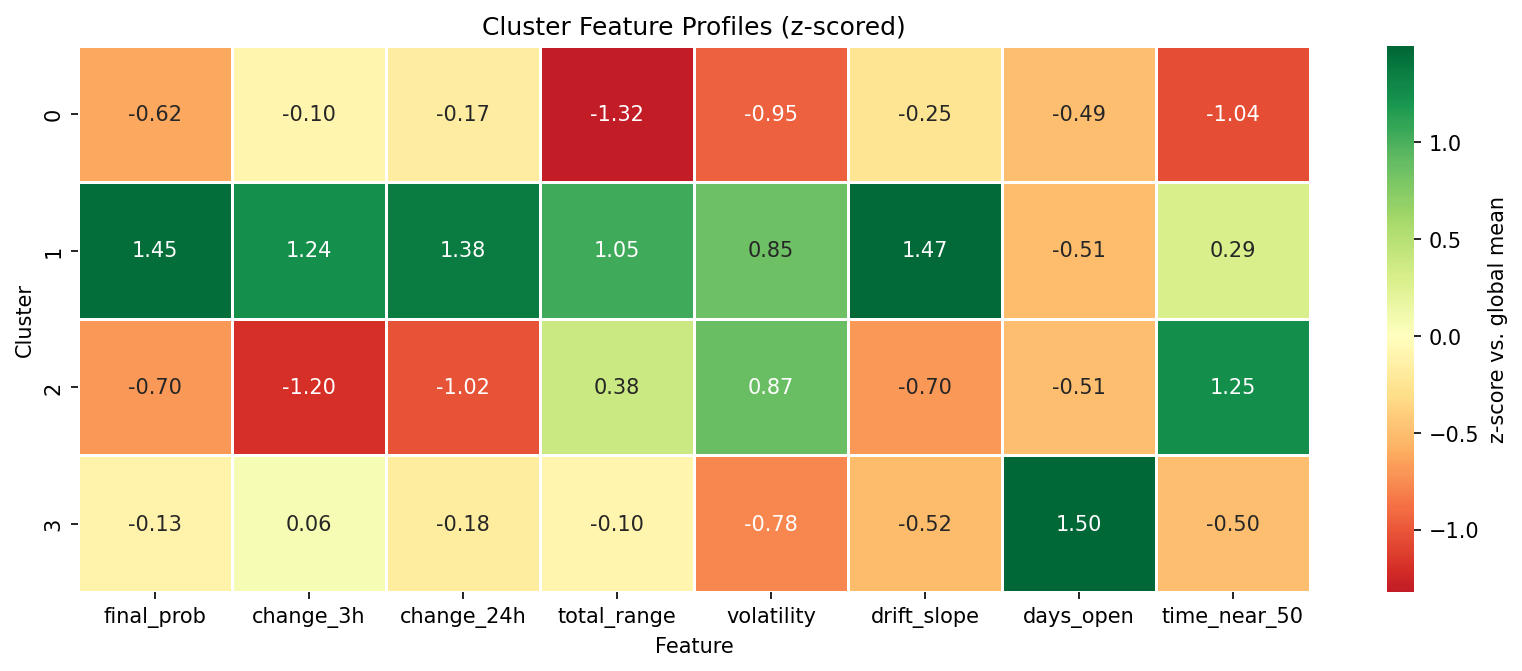
\includegraphics[width=\textwidth]{feature_heatmap.png}
\caption{Heatmap of z-scored cluster centroid values for each feature. Red = below average, green = above average relative to the full dataset. Cluster 1 stands out with high \texttt{change\_24h} and \texttt{total\_range}; Cluster 3 stands out with high \texttt{days\_open}.}
\end{figure}

% ─────────────────────────────────────────────────────────────────────────────
\section{Structural Analysis: Clusters vs.\ Market Type}

A key question is whether the behavioral clusters simply rediscover Kalshi's own taxonomy or reveal cross-cutting structure. We cross-tabulate cluster assignment against \texttt{market\_type}.

\begin{figure}[h!]
\centering
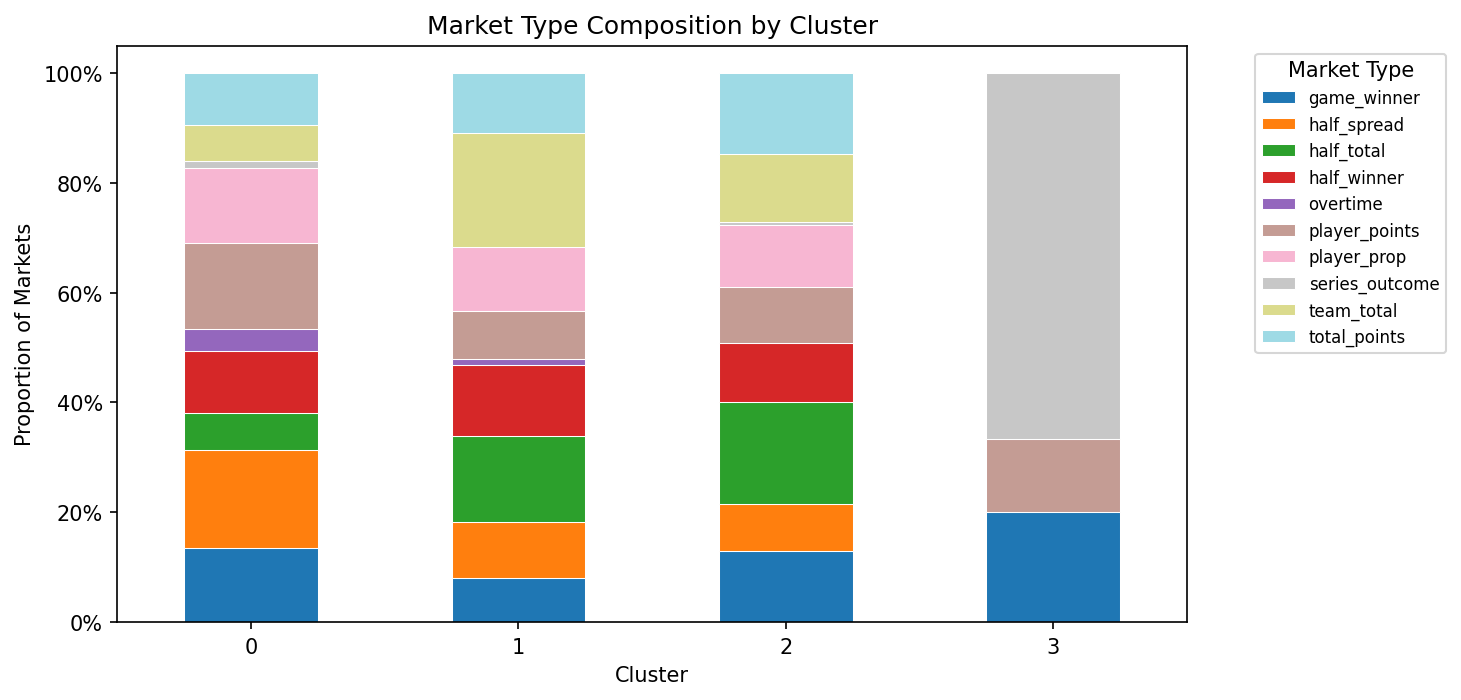
\includegraphics[width=0.85\textwidth]{sport_breakdown.png}
\caption{Composition of each cluster by Kalshi market type. Clusters contain mixtures of game outcomes, player props, totals, and spread markets — indicating that behavioral dynamics do not align with Kalshi's stated categories.}
\end{figure}

\textbf{Finding:} All four clusters contain a mix of market types. Cluster 0, for example, includes both half-spread and player-prop markets — they share behavioral similarity (consistent underdog pricing, low volatility) despite representing fundamentally different bets. This confirms that price dynamics cut \textit{across} Kalshi's taxonomy. Behavioral type is not determined by market category.

% ─────────────────────────────────────────────────────────────────────────────
\section{Mispricing Analysis}

\subsection{Methodology}
For each cluster $k$, let $n_k$ be the number of markets, $\bar{p}_k$ the mean final price (implied YES probability), and $y_k$ the number of YES resolutions. We define mispricing as:
\[
\delta_k = \frac{y_k}{n_k} - \bar{p}_k
\]
A well-calibrated cluster has $\delta_k \approx 0$. We test the null hypothesis of calibration using a two-sided binomial test:
\[
H_0: P(\text{YES}) = \bar{p}_k \quad \text{vs.} \quad H_1: P(\text{YES}) \neq \bar{p}_k
\]
Under $H_0$, $y_k \sim \mathrm{Binomial}(n_k,\, \bar{p}_k)$. We compute exact $p$-values using \texttt{scipy.stats.binomtest}.

\subsection{Results}

\begin{table}[h!]
\centering
\caption{Mispricing analysis results by cluster}
\begin{tabular}{crrrrrc}
\toprule
Cluster & $n$ & Avg.\ Final Prob & YES Rate & Mispricing & $p$-value & Sig.? \\
\midrule
0 & 453 & 0.163 & 0.141 & $-$0.021 & 0.227 & No \\
1 & 286 & 0.854 & 0.839 & $-$0.015 & 0.503 & No \\
2 & 177 & 0.138 & 0.158 & $+$0.020 & 0.444 & No \\
3 &  30 & 0.328 & 0.267 & $-$0.061 & 0.563 & No \\
\bottomrule
\end{tabular}
\end{table}

\begin{figure}[h!]
\centering
\begin{subfigure}[b]{0.49\textwidth}
  \centering
  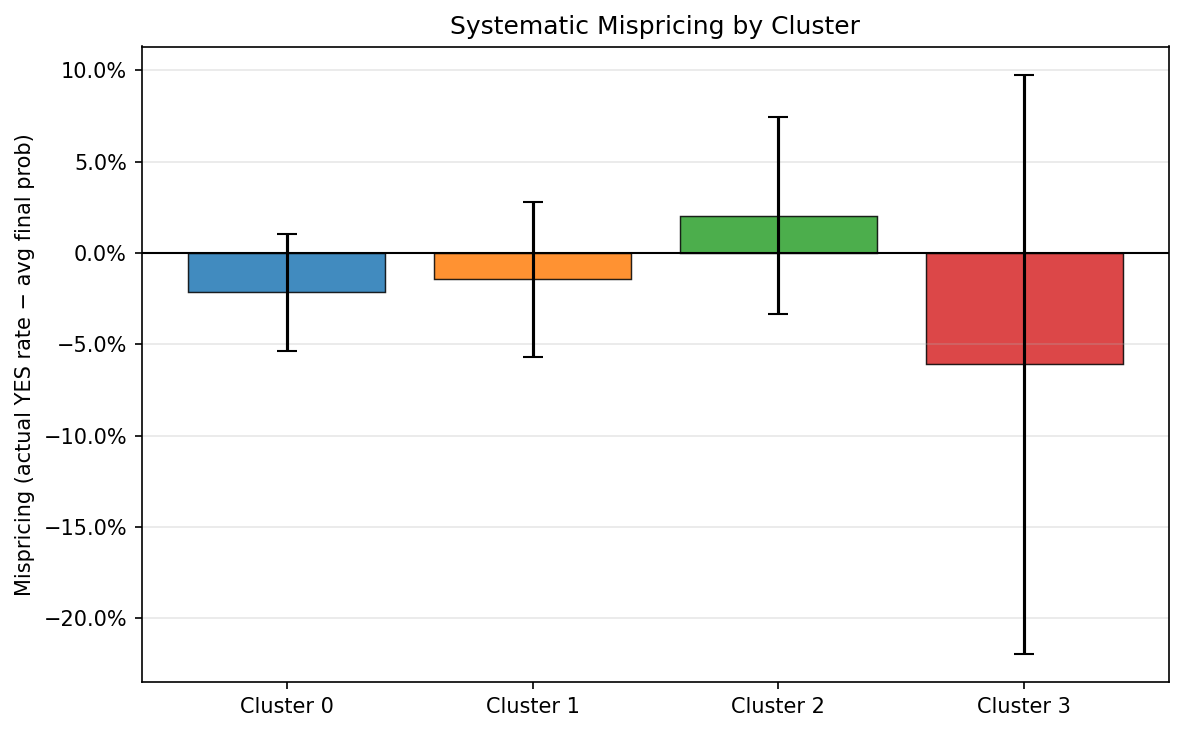
\includegraphics[width=\textwidth]{mispricing_chart.png}
  \caption{Mispricing per cluster with 95\% Wald confidence intervals.}
\end{subfigure}
\hfill
\begin{subfigure}[b]{0.49\textwidth}
  \centering
  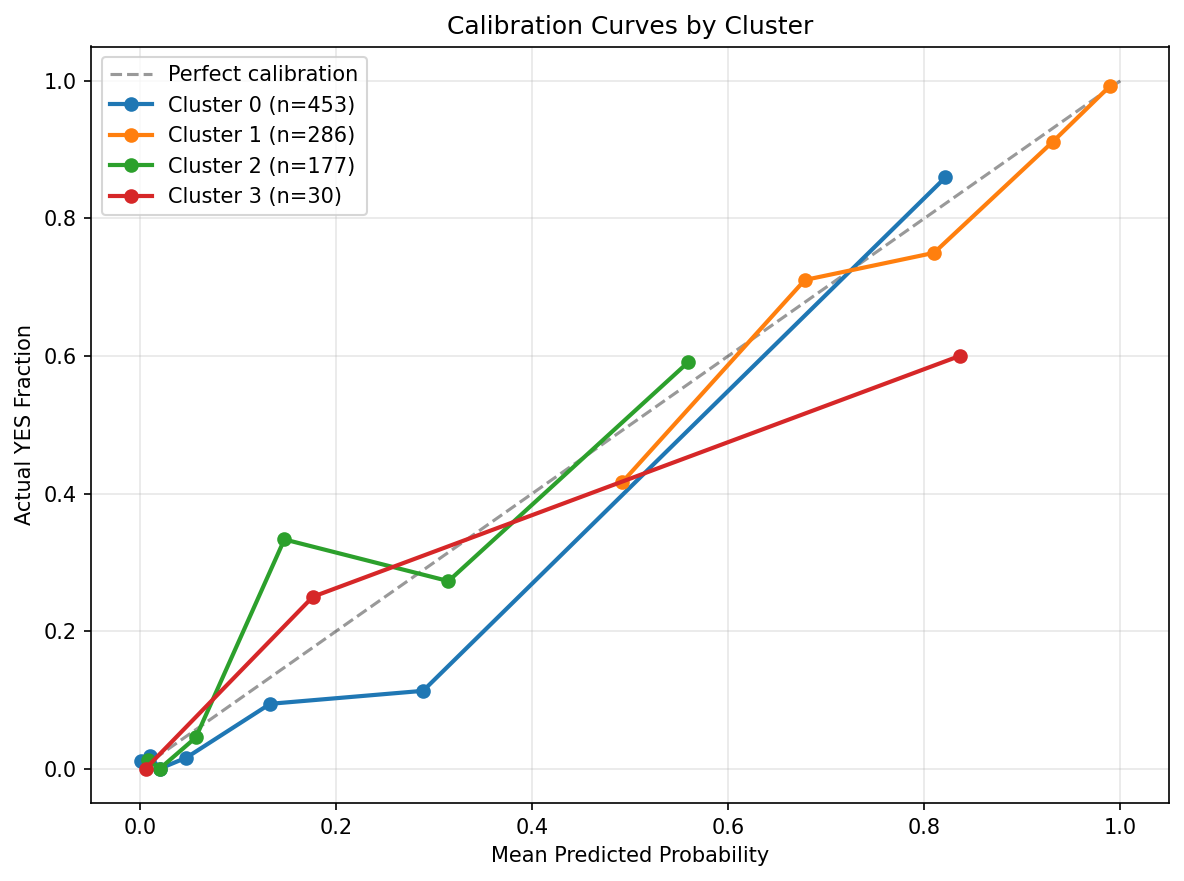
\includegraphics[width=\textwidth]{calibration_curve.png}
  \caption{Calibration curves per cluster. The dashed diagonal is perfect calibration.}
\end{subfigure}
\caption{Mispricing and calibration results.}
\end{figure}

\subsection{Interpretation}
No cluster exhibits statistically significant mispricing at the $\alpha = 0.05$ level. The largest absolute mispricing is Cluster 3 ($\delta_3 = -0.061$), but with only 30 markets the test has low power. The calibration curves confirm that prices track outcomes reasonably well across the probability range.

\textbf{Statistical power caveat:} Absence of significance is not proof of absence of edge. A true mispricing of 3 percentage points in Cluster 0 ($n=453$) would yield a standard error of approximately $\sqrt{0.163 \times 0.837 / 453} \approx 0.018$, giving a $z$-score of $\approx 1.7$ — below the $z=1.96$ threshold for $\alpha=0.05$. Detecting mispricing at this scale reliably would require several thousand markets. Our dataset is insufficient to rule out small but exploitable edges.

% ─────────────────────────────────────────────────────────────────────────────
\section{Conclusion}

\subsection{Summary of Findings}
\begin{enumerate}[noitemsep]
  \item \textbf{K-means with $k=4$ reveals four behaviorally distinct market types} based purely on pre-resolution price dynamics: stable underdogs, late-converging favorites, volatile near-misses, and long-duration series markets.
  \item \textbf{Behavioral clusters cut across Kalshi's market taxonomy.} Markets classified as game winners, player props, and team totals co-occupy the same behavioral clusters, indicating that price path dynamics are not determined by market category.
  \item \textbf{No statistically significant mispricing detected.} Kalshi markets appear well-calibrated at the cluster level — the crowd's final prices are consistent with observed resolution rates.
\end{enumerate}

\subsection{Limitations}
\begin{itemize}[noitemsep]
  \item \textbf{Single season:} Data covers one NBA season; behavioral patterns may vary across seasons.
  \item \textbf{Stratified sample:} We capped at 300 markets per type; some types may be underrepresented.
  \item \textbf{No out-of-sample validation:} Cluster assignments are descriptive; we do not test whether clusters trained on one period predict behavior in another.
  \item \textbf{Low power for mispricing:} Our sample is too small to detect mispricing below $\sim$3 percentage points.
  \item \textbf{No transaction costs:} Any apparent edge would be further reduced by Kalshi's spread and fees.
\end{itemize}

\subsection{Future Work}
Natural extensions include: multi-season analysis, out-of-sample cluster stability, incorporating volume as a feature, and testing whether Cluster 2 (volatile near-misses with $+2$ pp mispricing) shows significant edge in a larger dataset.

% ─────────────────────────────────────────────────────────────────────────────
\begin{thebibliography}{9}

\bibitem{wolfers2004}
Wolfers, J.\ \& Zitzewitz, E.\ (2004).
Prediction markets.
\textit{Journal of Economic Perspectives}, 18(2), 107--126.

\bibitem{arrow2008}
Arrow, K.\ et al.\ (2008).
The promise of prediction markets.
\textit{Science}, 320(5878), 877--878.

\bibitem{lloyd1982}
Lloyd, S.\ P.\ (1982).
Least squares quantization in PCM.
\textit{IEEE Transactions on Information Theory}, 28(2), 129--137.

\bibitem{rousseeuw1987}
Rousseeuw, P.\ J.\ (1987).
Silhouettes: A graphical aid to the interpretation and validation of cluster analysis.
\textit{Journal of Computational and Applied Mathematics}, 20, 53--65.

\bibitem{pedregosa2011}
Pedregosa, F.\ et al.\ (2011).
Scikit-learn: Machine learning in Python.
\textit{Journal of Machine Learning Research}, 12, 2825--2830.

\bibitem{kalshi2024}
Kalshi Inc.\ (2024).
Kalshi Trade API v2 Documentation.
\url{https://trading-api.readme.io/}

\end{thebibliography}

\end{document}
